\chapter{Magnetic vortex effects on the first-order reversal curve (FORC) diagram of greigite dispersions}
\label{ch:res-3}
\fancyhead[L]{Single-vortex effects on FORC diagrams}
\fancyhead[C]{}
\fancyhead[R]{}
\fancyfoot[C]{\thepage}

\section*{Abstract}
First-order reversal curve (FORC) diagrams are an increasingly used technique in geophysics that allows magnetic domain state identification. Since a magnetic particle's domain state is highly sensitive on the particle size, FORC diagrams provide a magnetic proxy for magnetic particles' size distributions. However, the FORC signal of particles with nonuniform magnetisations, which are the main carrier of natural remanent magnetisations in many systems, is still poorly understood. In this study, the properties of non-interacting, randomly oriented dispersions of greigite (Fe$_3$S$_4$) in the near uniform single-domain (SD) to single-vortex (SV) size range are investigated via micromagnetic calculations. The FORC diagrams were found to be highly sensitive to the magnetic domain state of the particles. The SD signal ($<50\nm$) was found to be in excellent agreement with previous SD coherent-rotation studies. A transitional range from $\roughly$50$\nm$ to $\roughly$70$\nm$ was identified for which a mixture of SD and SV behaviour during hysteresis produces complex FORC diagrams. Particles $> \roughly 70\nm$ show a purely SV behaviour with the remanent state for all particles in the ensemble a vortex state. It is found that for SV ensembles the FORC diagram provides a map of vortex nucleation and annihilation fields and the FORC distribution peak should not be interpreted simply as the coercivity of the sample, but as a vortex annihilation field on the path to saturation.\par

\section{Introduction}
First-order reversal curve (FORC) diagrams are a powerful tool in rock magnetic studies which allow for mineral and domain state identification as well as quantification of magnetostatic interactions between particles \citep{Pike1999,Roberts2000,Roberts2014,Dumas2007,Egli2010}. As such, they have been the subject of numerical studies aiming to relate the individual behaviour of the magnetic particles and small assemblages to the experimental bulk properties \citep{Pike1999,Carvallo2003,Carvallo2006,Muxworthy2004,Muxworthy2005,Newell2005,Harrison2014,ValdezGrijalva2017}.\par

With the exception of \citet{Carvallo2003}, all of these previous numerical studies have concentrated on the FORC diagrams of ideal, uniform single-domain (SD) particles. They have shown that uniaxial SD particles have patterns \citep{Muxworthy2004,Newell2005}, that are distinct from SD materials with cubic anisotropy \citep{Muxworthy2004,ValdezGrijalva2017}. However, it is well-documented that most natural systems have magnetic signals dominated by larger grains with more complex magnetic domain states, e.g., pseudo-single domain \citep{Dunlop}. Grains just above the SD threshold (e.g., $\roughly 64 \nm$ for magnetite, $\roughly 54 \nm$ for greigite), are typically in a single-vortex (SV) state. The SV state dominates magnetic structures over an order of magnitude \citep{Nagy2017, ValdezGrijalva2017B}, a range much wider than the stable SD range. SV grains have recently been found to be geologically meta-stable and retain relatively high remanences \citep{Nagy2017, ValdezGrijalva2017B}.\par

Previous experimental studies on nano-patterned arrays of SV particles \citep{Pike1999B,Dumas2007} found that the SV FORC diagrams are significatively more complex than the SD signal, displaying complex off-axis ``butterfly'' patterns that were related to vortex nucleation/annihilation processes. However, it is hard to relate the behaviour of 2D nano-patterned arrays to the behaviour of natural systems.\par

In natural samples, particles with varying size and orientations are dispersed in 3 dimensions. Thus, it is important to understand the contribution of dispersions of randomly aligned SV particles to FORC diagrams. Numerical modelling can aid the study of such systems. \citet{Carvallo2003} used a finite-difference model to calculate the FORC distributions of SV magnetite particles, however, their model was too low resolution to now be considered reliable, did not study random distributions nor did it model realistic grain morphologies.\par

In this study, we employ a micromagnetic finite element method (FEM) to study the FORC diagram properties of non-interacting ensembles of SD and SV greigite (Fe$_3$S$_4$). Greigite is the iron-sulphide counterpart to magnetite. Recent interest in greigite comes from both its promising properties for material scientists \citep{Li2014} and the abundance of this mineral in sedimentary rocks for Earth scientists \citep{Roberts2011}; FORC diagrams are often used to help identify greigite. The relatively high anisotropy of greigite means that the behaviour of this mineral is representative of cubic-anisotropic ferromagnets like magnetite or iron. We obtain FORC diagrams of non-interacting dispersions of randomly oriented greigite with sizes 30--80$\nm$; this size range covers the SD--SV threshold \citep{ValdezGrijalva2017B}. The unstructured discretisation of FEMs allows us to study realistic shapes of greigite particles observed in nature. We determine the onset of SV behaviour and its consequences for FORC diagram interpretation.\par
%-----------------------------------------------------

\section{Methodology}
\subsection{The micromagnetic algorithm}
A ferromagnetic material{\textemdash}neglecting thermal and magnetostrictive effects{\textemdash}has a Gibbs free-energy functional given by \citep{Brown}
{\par\nobreak\noindent}
\begin{equation}
E_\text{G} = \int_{\Omega} (\phi_{\text{exchange}} + \phi_{\text{anisotropy}} + \phi_{\text{stray}} + \phi_{\text{external}})\,\text{d}^3 \boldsymbol{r},
\end{equation}
with $\Omega$ the ferromagnetic volume. Here,
{\par\nobreak\noindent}
\begin{equation}
\phi_{\text{exchange}}=A|\nabla\boldsymbol{m}|^2
\end{equation}
 with the reduced magnetisation vector $\boldsymbol{m}$ and the exchange stiffness constant $A$, is the expression for the energy density due to the quantum-mechanical exchange forces \citep{Landau1935}.
{\par\nobreak\noindent}
\begin{equation}
\phi_{\text{anisotropy}}=\frac{K_1}{2}\sum_{i\neq j}\gamma_i^2\gamma_j^2 + K_2\prod_i\gamma_i^2,
\end{equation}
with $\gamma_i$ the direction cosines and $K_1, K_2$ the first and second magnetocrystalline anisotropy (MCA) constants, is the MCA energy density in the cubic anisotropy system. In terms of the reduced magnetisation vector components this becomes:
{\par\nobreak\noindent}
\begin{equation}
\phi_{\text{anisotropy}}=K_1(m_x^2m_y^2+m_y^2m_z^2+m_z^2m_x^2),
\end{equation}
where $K_2$ has been neglected since $K_1$ is the dominant term at room temperature. The magnetostatic self-energy density is given by
{\par\nobreak\noindent}
\begin{equation}
\phi_{\text{stray}}=-\frac{\mu_0M_\text{S}}{2}\boldsymbol{m}\cdot\boldsymbol{H}_{\text{stray}},
\end{equation}
with $\boldsymbol{H}_{\text{stray}}$ the stray field produced by the ferromagnetic body and $M_\text{S}$ the saturation magnetisation. Finally, the energy density due to an external magnetic field $\boldsymbol{H}_{\text{external}}$ is
{\par\nobreak\noindent}
\begin{equation}
\phi_{\text{external}}=-\mu_0M_\text{S}\boldsymbol{m}\cdot\boldsymbol{H}_{\text{external}}.
\end{equation}\par

It is known that the system will be spontaneously driven towards an equilibrium state with a locally minimal magnetic Gibbs free-energy \citep{Brown}. In this study we utilise a modified gradient descent method with the aim of finding the equilibrium magnetisation \citep{OConbhui2017}.\par

The discretisation of the spatial domain is achieved by a decomposition of the volume into tetrahedral elements. This allows for arbitrary geometries to be modelled. To model accurately nonuniform magnetisations the spatial discretisation in the model should be smaller than the exchange length $l_\text{exch.} = \sqrt{2A/\mu_0M_\text{S}^2}$ \citep{Rave1998}, which for greigite is $l_\text{exch.} \approx 6.6\, \text{nm}$; a maximum element size of 5$\nm$ has been chosen for all the models. The non-local problem of calculating the stray field is resolved by a hybrid finite-element/boundary-element formulation \citep{Fredkin1990}.\par

The magnetic parameters of greigite used in this investigation are: the saturation magnetisation $M_\text{S}=3.51\,\mu_\text{B}\,\text{p.c.u.}$ or $\roughly 2.7 \times 10^5\,\text{A/m}$ \citep{Li2014}; the exchange stiffness constant $A=2\times10^{-12}\,\text{J}/\text{m}$ \citep{Chang2008}; and the first MCA constant $K_1=-1.7\times10^4\,\text{J}/\text{m}^3$ \citep{Winklhofer2014}. This set of parameters has been used in recent numerical studies of greigite \citep{ValdezGrijalva2017B,ValdezGrijalva2017}.\par

\subsection{The FORC model}
FORC diagrams are constructed from a class of partial hysteresis curves called first-order reversal curves \citep{Mayergoyz1986}, each starting at a value $B_a$ of the applied field along the main hysteresis branch and tracing the magnetisation as the field $B_b$ is increased to saturation. A magnetisation function on two variables $M=M(B_a, B_b)$ is thus obtained. The FORC distribution $\rho$ is then defined as \citep{Roberts2000}:
{\par\nobreak\noindent}
\begin{equation}
\rho=-\frac{1}{2}\frac{\partial^2 M}{\partial H_a \partial H_b}=-\frac{\mu_0^2}{2}\frac{\partial^2 M}{\partial B_a \partial B_b},
\end{equation}
where $\mu_0$ is the magnetic constant (or vacuum permeability) and $H=B/\mu_0$.\par

Once $M(B_a, B_b)$ is obtained, the calculation of $\rho(B_a, B_b)$ is done by least-square fitting a degree 2 polynomial surface $a_0 + a_1 B_a + a_2 B_b + a_3 B_a B_b + a_4 B_a^2 + a_5 B_b^2 = 0$ on a subgrid of $M(B_a, B_b)$ centered around $(B_a, B_b)$ as determined by the so-called smoothing factor (SF) and including (2$\times$SF + 1)$^2$ points; the value of $\rho$ is then simply $-\mu_0^2 a_3/2$ \citep{Pike1999}. FORC diagrams are usually presented with rotated axes $B_c=(B_b - B_a)/2$, $B_u=(B_b + B_a)/2$.\par

Random orientation distributions were determined by taking 500 field orienations from a sector of the sphere (Fig. \ref{FIG_01}). We chose to use 500 field orientations as a good compromise between accuracy and calculation speed. Also, we note that for each particle/field-orientation the hysteresis curve consists mostly of reversible motion of the magnetisation; thus, we only need to calculate the main branch of the hysteresis loop and the few reversal curves starting at the different switching fields along the main branch \citep{ValdezGrijalva2017}. These simplifications vastly reduce the amount of calculations needed without loss of generality. The external-field rate of change for all models was 1$\mT$ with a saturation field of 250$\mT$ thus, 501 reversal curves were calculated for each particle/field-orientation.\par
\begin{figure}
\centering
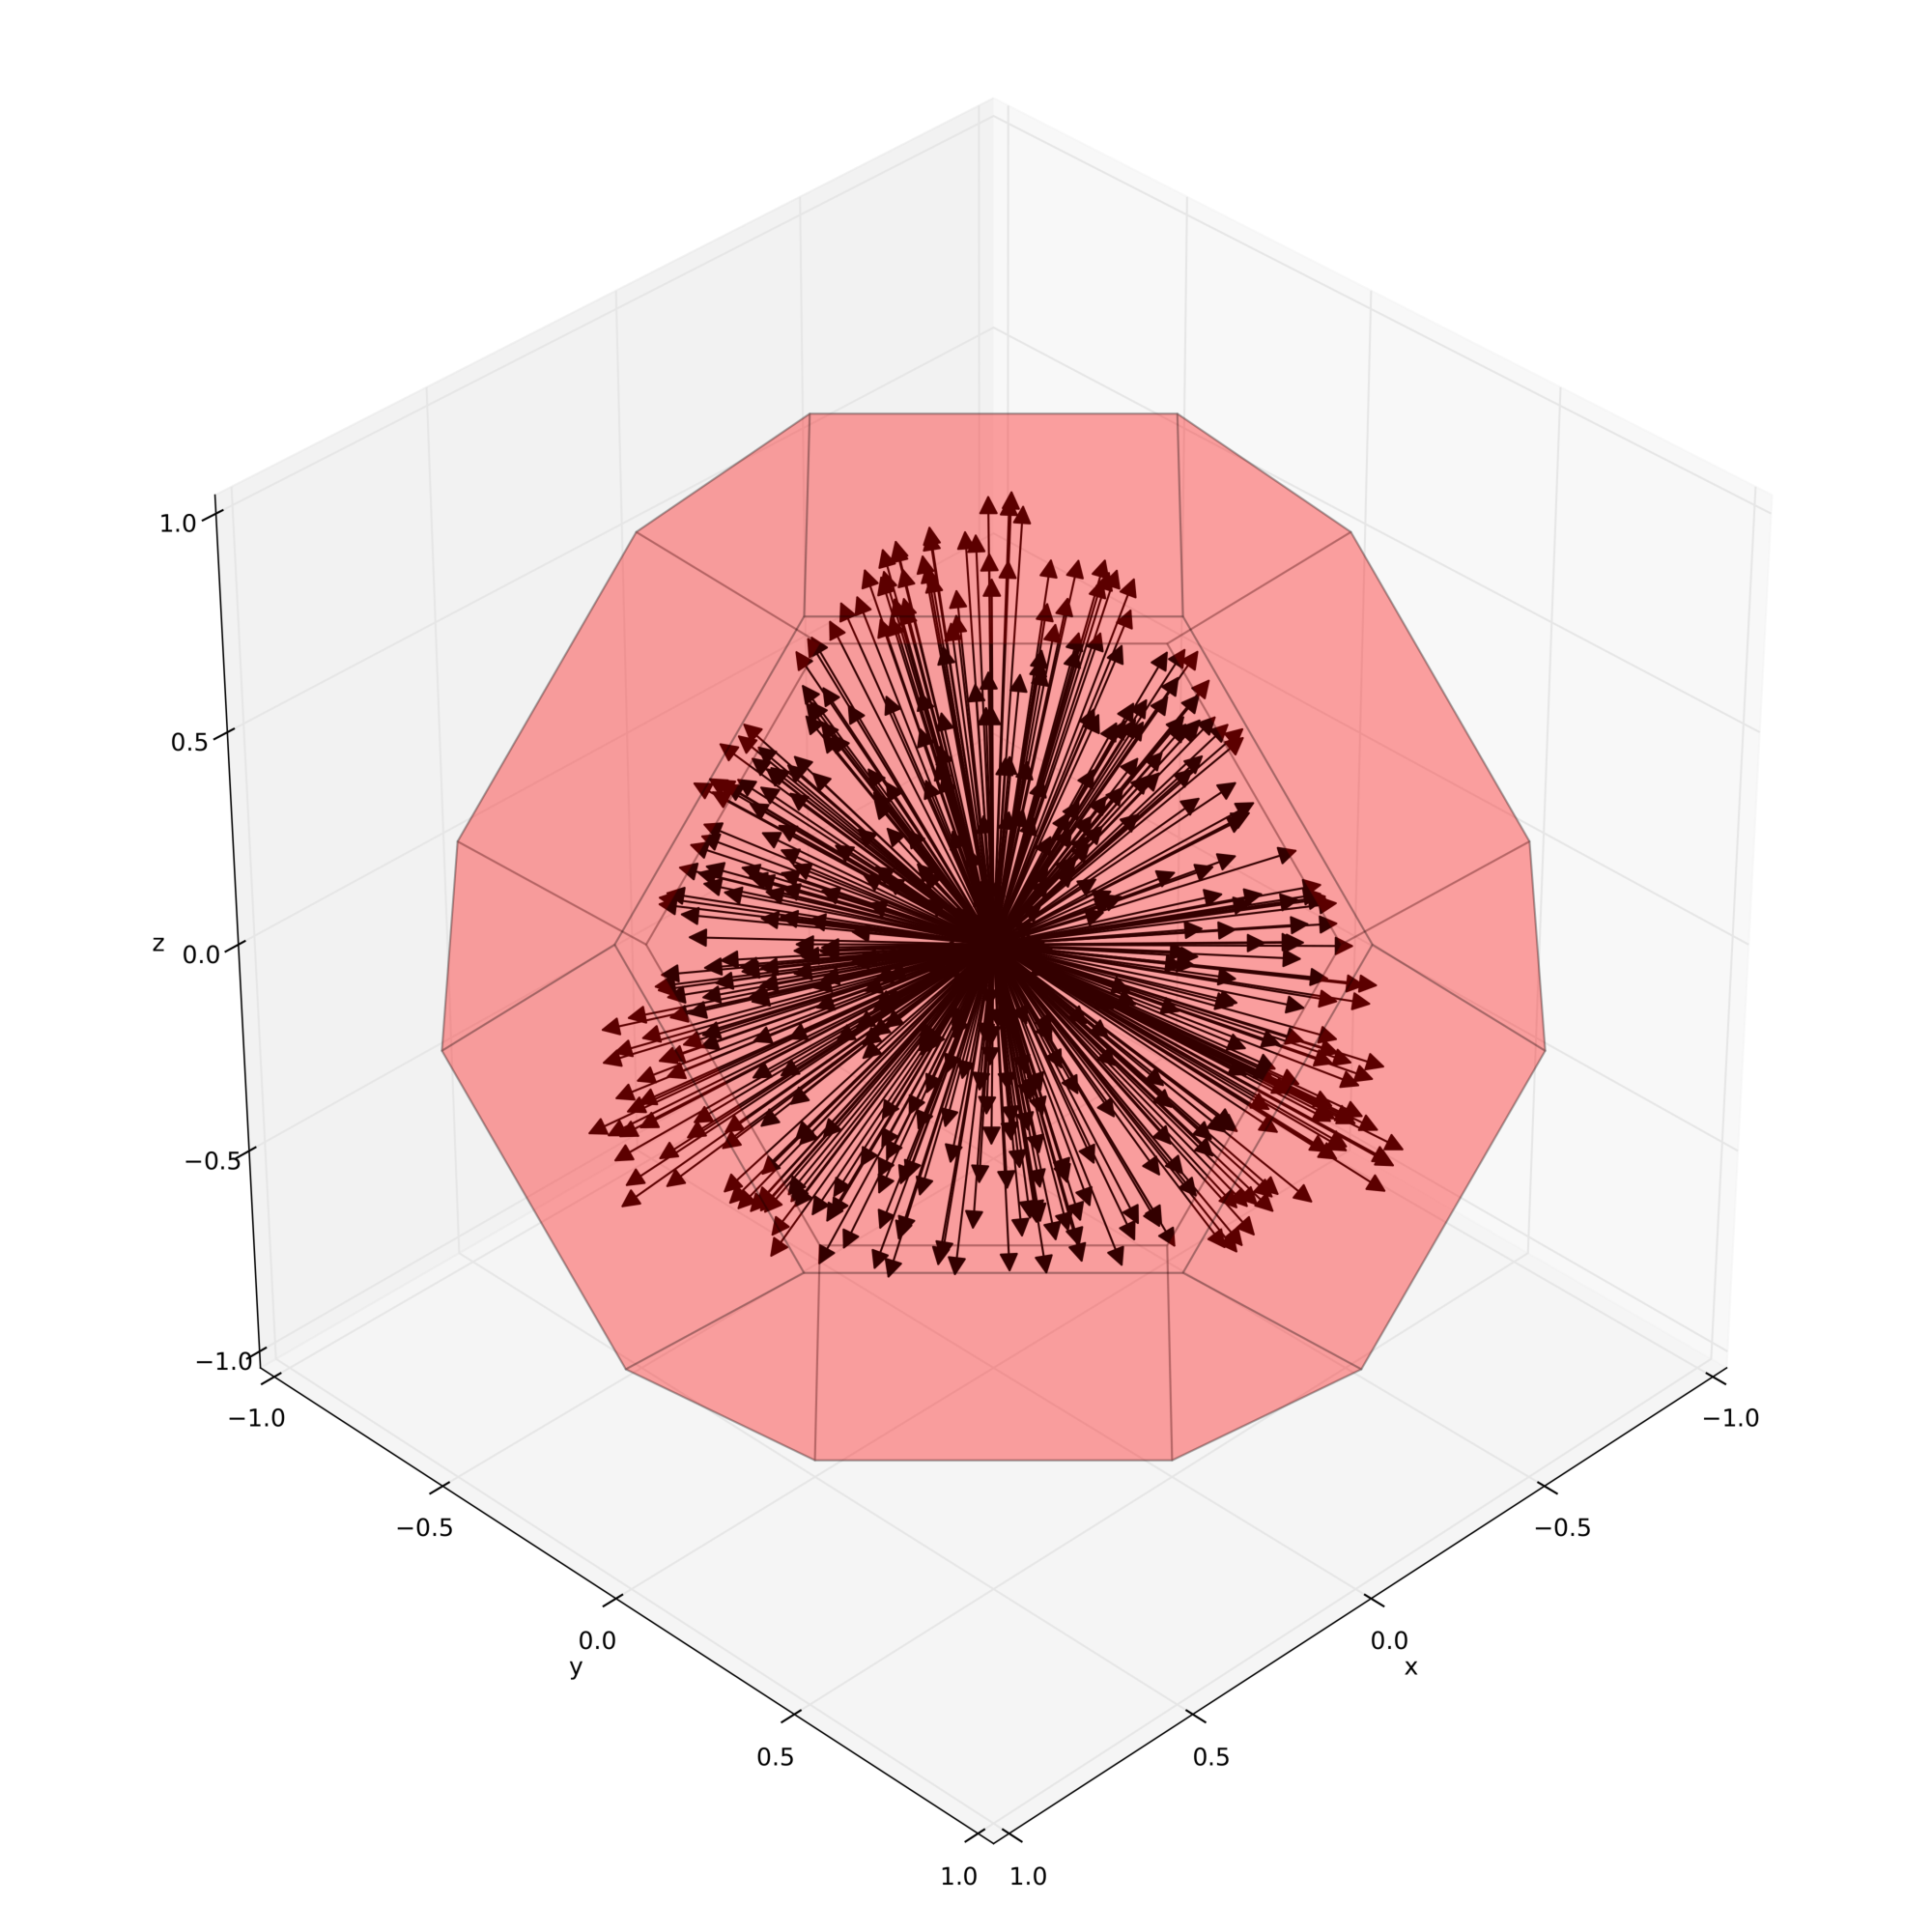
\includegraphics[width=\textwidth]{research-3/figs/FIG_01.pdf}
\caption[Model geometry and field orientations]{Model geometry and field orientations. The most common morphology for authigenic greigite is truncated octahedral. To avoid the high density of field orientations necessary near the sphere poles when using a regular grid, 500 random field orientations from a distribution uniform over a sector of the sphere were chosen. The periodicity of the magnetocrystalline anisotropy and particle symmetry allows to only model the effects of field orientations on a sector of the sphere without loss of generality.}
\label{FIG_01}
\end{figure}
Scanning electron microscopy and transmission electron microscopy micrographs of naturally occurring greigite samples \citep{Snowball1997,Vasiliev2008,Roberts2015} reveal that greigite tends to grow authigenically as well-defined regular truncated octahedral particles. Micromagnetic calculations for truncated octahedral greigite particles show the SD--SV threshold to be $\roughly 54\nm$ \citep{ValdezGrijalva2017B}. In this study we model the FORC diagram of non-interacting ensembles of truncated octahedral greigite particles sized 30--80$\nm$ (size normalised to the volume of a cube) every 2$\nm$ as this range covers the transition from SD to SV behaviour.\par

%-----------------------------------------------------

\section{Results}
For the ensembles with particles $<50\nm$ the hysteretic behaviour is dominated by SD particles with coherent rotations (Fig. \ref{FIG_02}). This is seen by comparing the FORC diagrams of these ensembles (Fig. \ref{FIG_02}b) with those of ``pure'' SD, coherent-rotating greigite particles (Fig. \ref{FIG_02}a) determined using the method outlined in \citet{ValdezGrijalva2017}. The diagrams for the particles $<50\nm$ obtained with the micromagnetic algorithm (Fig. \ref{FIG_02}b) are offset $\roughly 3\mT$ towards the left compared to the dipolar model (Fig. \ref{FIG_02}a); lower coercivities due to the micromagnetic algorithm including magnetostatic self-interaction effects as well as flowering (small deviations from a perfect SD structure) account for this effect.\par
\begin{figure}
\centering
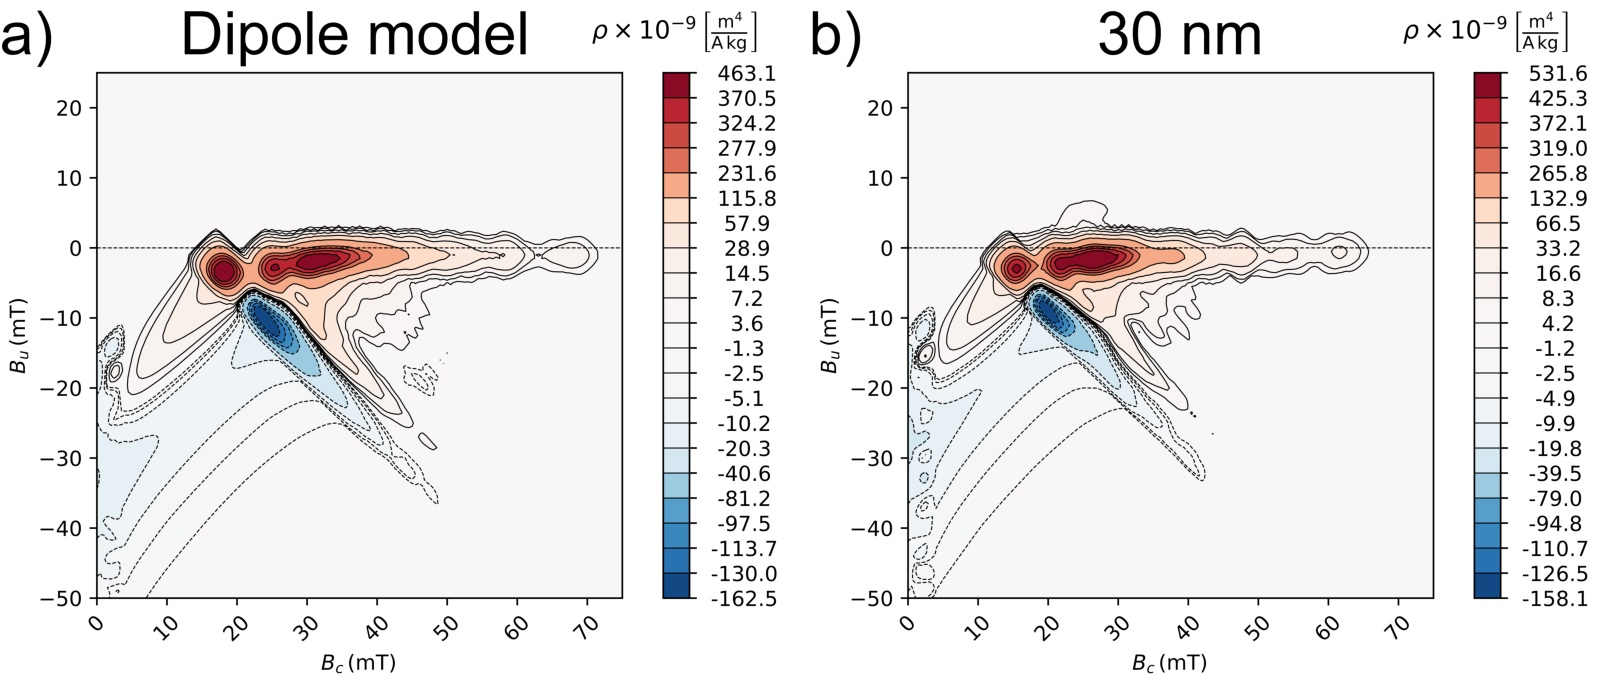
\includegraphics[width=\textwidth]{research-3/figs/FIG_02.pdf}
\caption[Comparison between dipole and micromagnetic model]{Comparison between dipole and micromagnetic model. a) Dipole model; the FORC diagram (SF=4) of a non-interacting ensemble of SD greigite obtained using the model of \citet{ValdezGrijalva2017}. b) Micromagnetic model; the FORC diagram (SF=4) of a non-interacting ensemble of 30$\nm$-sized truncated octahedral greigite particles. Up to 48$\nm$ the FORC diagram is that of an ensemble of coherent-rotating SD particles. For particles larger than 48$\nm$, magnetic vortex effects become noticeable.}
\label{FIG_02}
\end{figure}
Particles with cubic anisotropy exhibit hysteresis behaviour departing from the simple hysteron with one plus-state and one minus-state. There exist intermediate easy axis states along their hysteresis curves even when they are SD \citep{ValdezGrijalva2017}. The tilted, elongated, negative-valued ridge (Fig. \ref{FIG_02}) is a consequence of the cubic anisotropy and is produced by the fraction of particles with hard-axes closely aligned with the applied field. These particles have the lowest switching fields: from the plus-state to an intermediate state at $B= B^{+}_{*}$ and from the intermediate state to the minus-state at $B=B^{*}_{-}$. Reversal curves with $B^{*}_{-} < B_a < B^{+}_{*}$ experience a sharp upward discontinuity at $B_b = B^{*}_{+} < |B^{+}_{*}|$ when the hard-aligned particles return to the plus-state from their intermediate states. The combination of this type of irreversible events in the hard-aligned particles cause the local peak at $B_c\approx 15 \mT, B_u\approx {-}3\mT$ (Fig. \ref{FIG_02}b). On the reversal curves with $B_a < B^{*}_{-}$ the hard-aligned particles are initially in the minus-state and undergo irreversible rotation to an intermediate state on the path to positive saturation at $B=B^{-}_{*} = |B^{+}_{*}|$ due to the symmetry of the particles and the lack of magnetostatic interactions. The combination of these irreversible events causes a negative FORC distribution source at $B_a=B^{*}_{-}, B_b=B^{*}_{+}$. The sum effect of this type of sources for many particles with a distribution of switching fields produces the elongated negative contribution observed in all SD ensembles.\par

The fraction of particles with easy axis alignment close to the applied field orientation exhibit hysteron-like behaviour, i.e., just two switching fields: from the plus-state to the minus-state $B^{+}_{-}$ and viceversa $B^{-}_{+}$. The lack of interactions and symmetry of the particles ensure that $|B^{+}_{-}| = B^{+}_{-}$. Thus, this fraction of particles produce FORC distribution sources at $B_a=B^{+}_{-}, B_b=B^{-}_{+}$. These type of sources accumulate on the line $B_a=-B_b$. This type of irreversible events account for the most drastic changes in the magnetisation of the ensemble and thus account for the high slopes around the coercive field of the sample. This makes the position of the FORC diagram peak coincide with the coercivity $B_\text{C}\approx 24\mT$ of the SD ensembles.\par

Particles with size $d \geq 50\nm$ switch incoherently; the FORC diagrams depart from coherent rotation SD-like behaviour as the tight boomerang-shaped FORC diagram pattern exhibited by the SD greigite becomes more fragmented (Fig. \ref{FIG_03}). This change is initially driven by the particles with hard axes close to the applied field nucleating hard-aligned vortices \citep{ValdezGrijalva2017B} as intermediate meta-stable states during hysteresis. Even though the nucleation of hard-aligned vortices is taking place for particles with sizes below the zero-field SD--SV threshold $d_0\approx 54\nm$ \citep{ValdezGrijalva2017B}, this is expected as the nucleation of a vortex greatly reduces the Gibbs free-energy. A corollary of this is that a fraction of particles (those with easy axis alignment close to the applied field) above the zero-field SD--SV threshold can remain in a SD state during the entirety of hysteresis. These effects are due to the distortion of the zero-field energy landscape by the applied field.\par
\begin{figure}
\centering
\includegraphics[width=\textwidth]{research-3/figs/FIG_03.pdf}
\caption[FORC diagrams with increasing vortex effects]{FORC diagrams with increasing vortex effects. All diagrams with SF=4. a) 50$\nm$; b) 60$\nm$; c) 66$\nm$; d) 76$\nm$. At these sizes, an ever larger fraction of the particles begin to rotate via nonuniform magnetisations, i.e., vortex nucleation. At 76$\nm$ all particles are in the single vortex remanent state.}
\label{FIG_03}
\end{figure}
An appreciable positive source in the FORC distribution appears along the $B_u=0$ axis at $B_c\approx 52\mT$ ($B_c$ axis not to be confused with the coercivity $B_\text{C}$) for the ensembles with particles $\geq 54\nm$ (Fig. \ref{FIG_04} region 5); this contribution represents the annihilation of vortex states on the return to positive saturation. The elongated, negative ridge of the SD diagram and its corresponding symmetric positive source move towards lower values of $(B_c, B_u)$ (Fig. \ref{FIG_04} regions 1, 3) and the first sources for $B_u > 0$ begin to form (Fig. \ref{FIG_04} region 2); these are elongated features at a 45 degree angle from the $B_u=0$ axis, different from the vertical widening usually attributed to the presence of magnetostatic interactions \citep{Muxworthy2004,Muxworthy2005}.\par
\begin{figure}
\centering
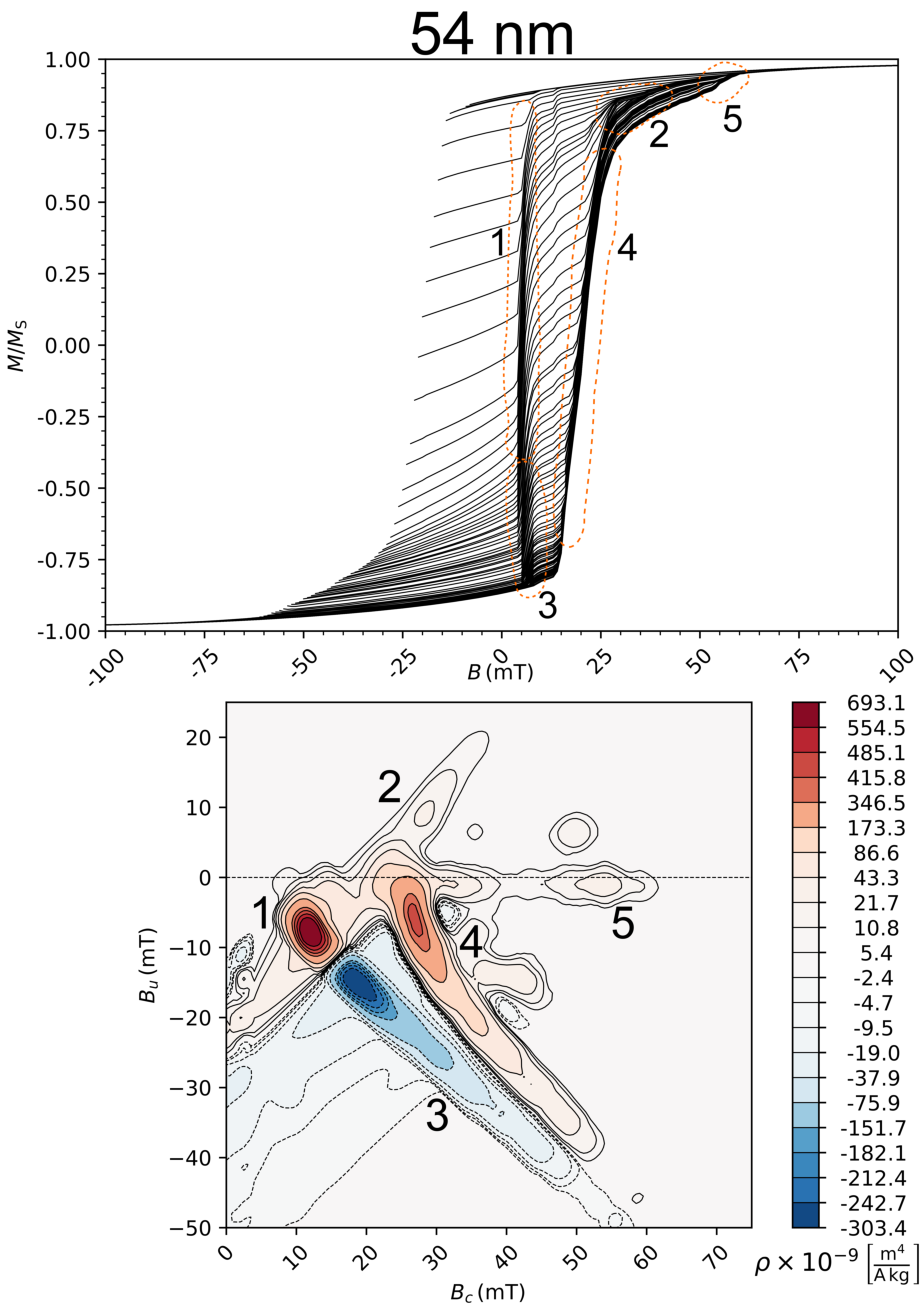
\includegraphics[width=\textwidth]{research-3/figs/FIG_04.pdf}
\caption[FORC diagram and hysteresis curves of 54$\nm$-sized particles]{FORC diagram (SF=4) and hysteresis curves of 54$\nm$-sized particles. Annotations link the FORC diagram sources to the raw hysteresis curves. See text for a detailed relation.}
\label{FIG_04}
\end{figure}
For the particles slighly below and above the SD--SV threshold $d_0$, vortex nucleation occurs only for negative values of the applied field, thus the noticeable changes in the FORC diagram (Fig. \ref{FIG_03}a--c) are not reflected in changes in the (saturation) remanence $M_\text{RS}$ to saturation magnetisation $M_\text{S}$ ratio up to 72$\nm$, whereas the coercivities sharply decrease above 48$\nm$ (Fig. \ref{FIG_05}b). The monotonically-decreasing trend of the coercivites is preserved up to 62$\nm$ when the coercivity rises from $B_{\text{C}}\approx 15 \mT$ to $B_{\text{C}}\approx 20 \mT$ for $d=68\nm$.\par
\begin{figure}
\centering
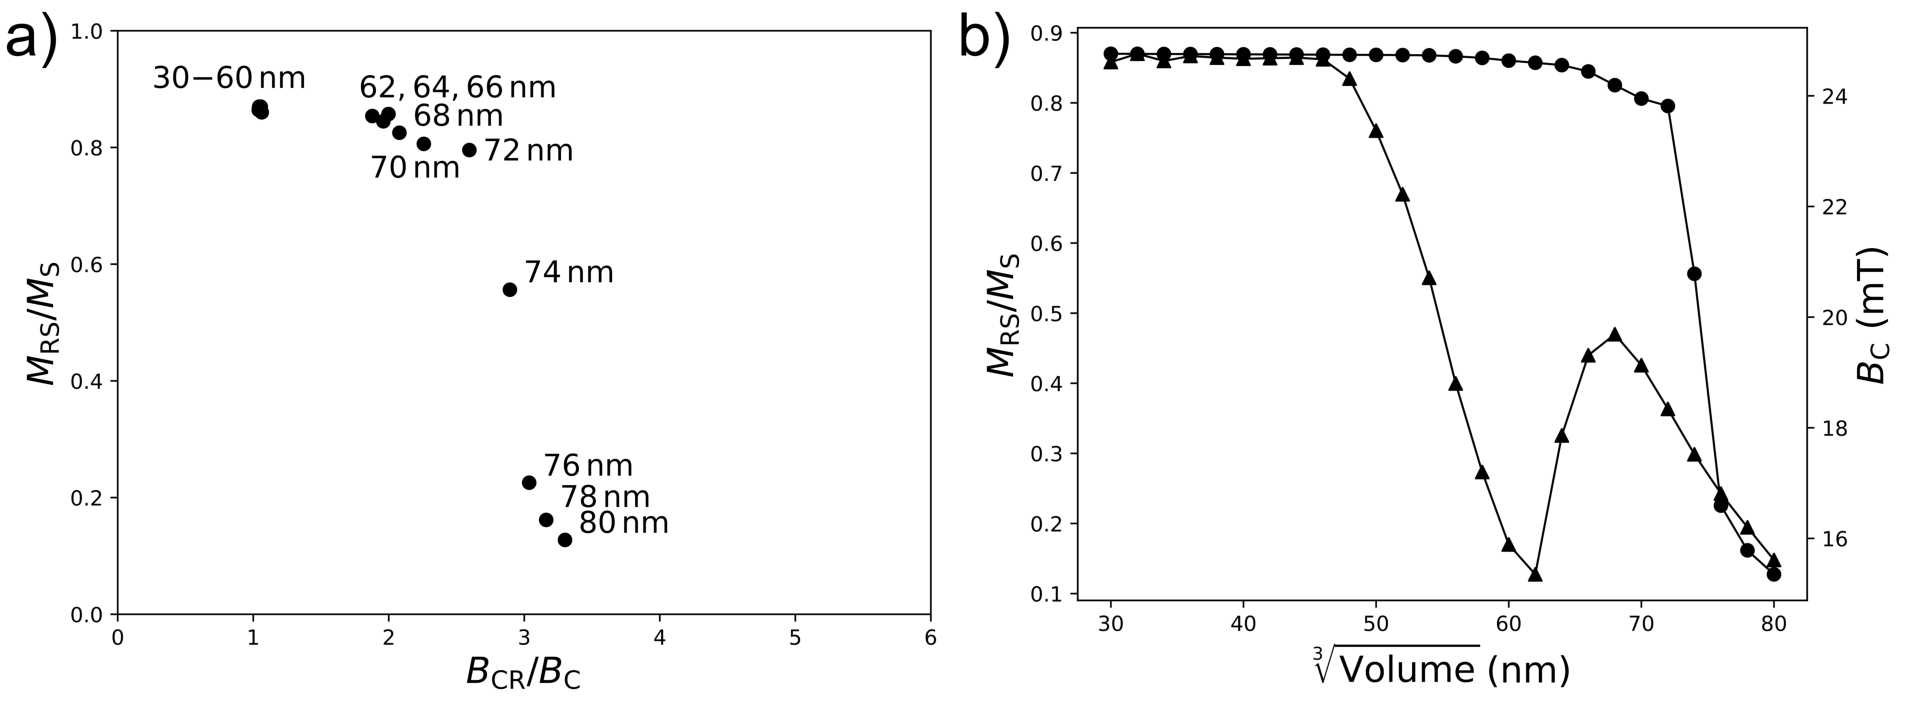
\includegraphics[width=\textwidth]{research-3/figs/FIG_05.pdf}
\caption[Day plot and remanence/coercivity against size]{Day plot and remanence/coercivity against size. a) The Day plot shows the particles up to 60$\nm$ to be SD; however, we know from the micromagnetic solutions that vortices are formed from 50$\nm$ onward. Particles sized 62$\nm$ to 72$\nm$ plot in an unexpected region. Particles larger than 74$\nm$ plot as PSD grains. b) Remanence (circles) and coercivity (triangles) against particle size.}
\label{FIG_05}
\end{figure}
On increasing size, the coercivities further decrease accompanied by a sharp decrease in $M_\text{RS}$ (Fig. \ref{FIG_05}b). The drop in $M_\text{RS}$ is driven by particles nucleating vortices at $B_a>0$ for $d \geq 68\nm$. For $d \geq 76\nm$, all particles nucleate vortices which become the remanent magnetic domain state; this is reflected in the Day plot \citep{Day1977}, a scatter plot of the $M_\text{RS}/M_\text{S}$ ratio against the coercivity of remanence $B_\text{CR}$ (the field necessary to demagnetise the remanence) to $B_\text{C}$ ratio by the particles sized 76$\nm$ and larger plotting in the region usually designated as pseudo single-domain (PSD) (Fig. \ref{FIG_05}a), synonymous with SV in this paper.\par

Particles sized 62--72$\nm$ move away from the Day plot region usually attributed to SD grains (Fig. \ref{FIG_05}a) to a region with high remanence but larger values of $B_{\text{CR}}/B_{\text{C}}$ ratio. These sizes coincide with the anomalous behaviour of the coercivity rising for these sizes (Fig. \ref{FIG_05}b). The increased coercivities can be explained by the nucleation of vortices causing the hysteresis loop to become increasingly wasp-waisted (Fig. \ref{FIG_06}) and thus cross the zero-magnetisation axis at increasing (absolute) values of the applied field strength. The FORC diagrams for these sizes are the most complex of all, showing a variety features (Figs. \ref{FIG_03}c, \ref{FIG_06}) caused by the complex interplay of SV and SD effects. The elongated, negative ridge becomes more faint with increasing particle size. Whereas, the positive sources for $B_u>0$ become larger and move towards the $B_c=0$ axis with size. Large, positive FORC distribution sources for $B_u>0$ along the $B_c=0$ axis are expected for the larger multi-domain (MD) grains \citep{Roberts2006}, and this behaviour is representative of that tendency.\par
\begin{figure}
\centering
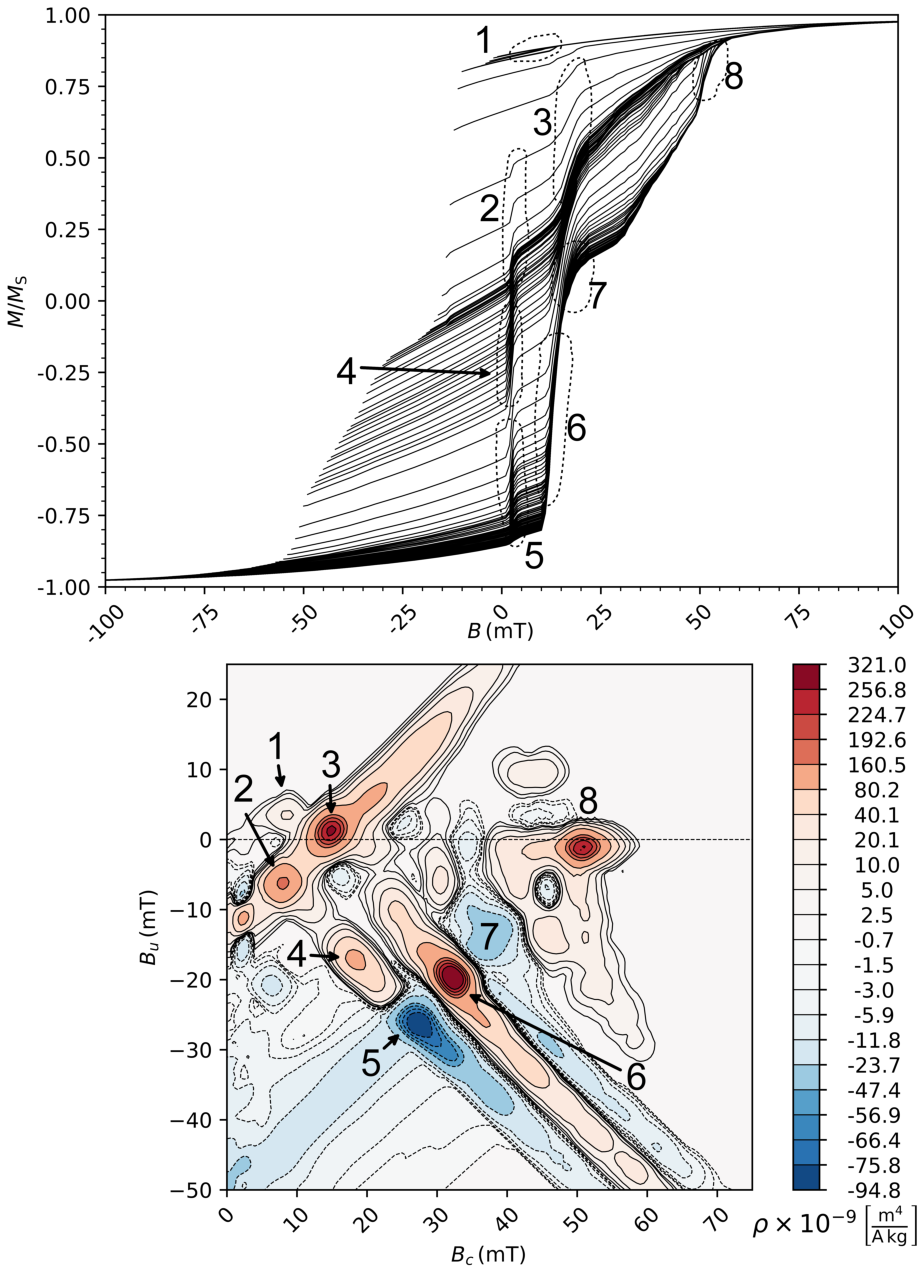
\includegraphics[width=\textwidth]{research-3/figs/FIG_06.pdf}
\caption[FORC diagram and hysteresis curves of 62$\nm$-sized particles]{FORC diagram (SF=4) and hysteresis curves of 62$\nm$-sized particles. Annotations link the FORC diagram sources to the raw hysteresis curves. See text for a detailed relation.}
\label{FIG_06}
\end{figure}
The non-interacting nature of these ensembles means that the SD and SV FORC signals are linearly additive. Therefore, it is possible to discern the FORC sources due to SD particles (Fig. \ref{FIG_06}, regions 3, 6) and to SV particles (Fig. \ref{FIG_06}, regions 1, 2, 4, 5, 7, 8).\par

The elongated, negative ridge typical of cubic magnetocrystalline anisotropy (MCA) SD particles \citep{ValdezGrijalva2017} disappears for the particles $\geq 76 \nm$ (Fig. \ref{FIG_03}d). A symmetric negative feature near the origin becomes larger and of a magnitude comparable to the largest positive sources. For $d=76$ and 78$\nm$ the negative source is larger (absolute value) than the distribution peak (Fig. \ref{FIG_03}d). For the 80$\nm$ particle model, a faint negative source appears close to the $B_u=0$ axis (Fig. \ref{FIG_07} region 6). Fig. \ref{FIG_07} represents the contribution of purely SV particles, that is, ensembles of particles that are all in a single vortex remanent state. It is logical that these are somewhat less complex than the diagrams of ensembles comprised of a fraction of particles still in the SD state as well as some in the SV state; the difference is due to the field angle relative to the particle orientation.\par
\begin{figure}
\centering
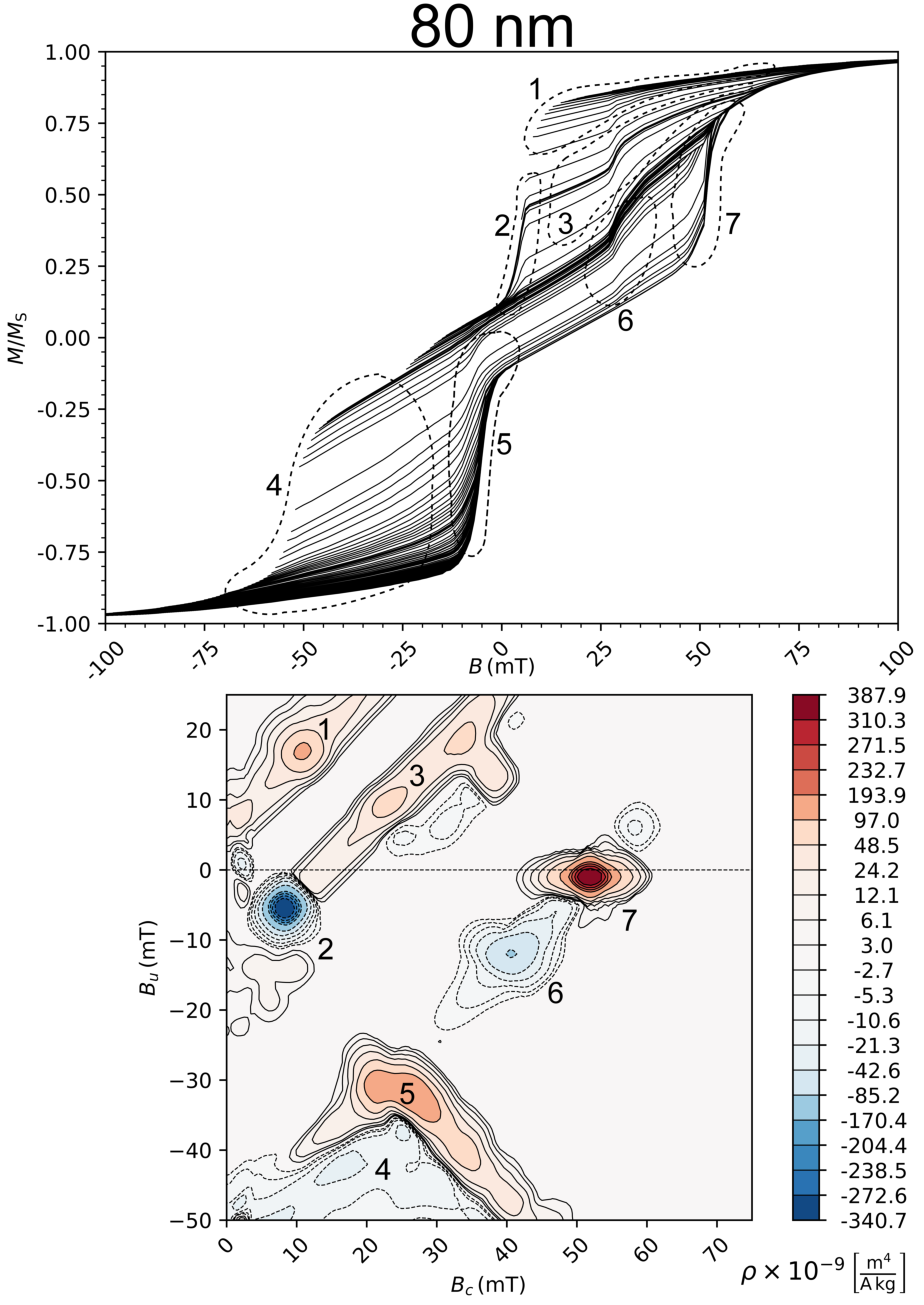
\includegraphics[width=\textwidth]{research-3/figs/FIG_07.pdf}
\caption[FORC diagram and hysteresis curves of 80$\nm$-sized particles]{FORC diagram (SF=4) and hysteresis curves of 80$\nm$-sized particles. Annotations link the FORC diagram sources to the raw hysteresis curves. See text for a detailed relation.}
\label{FIG_07}
\end{figure}
Particles with hard axes closely aligned with the applied field nucleate hard-aligned vortices at high values of the applied field (Fig. \ref{FIG_08}); as the field is decreased below $\roughly 12\mT$ these vortices irreversibly rotate to an easy axis alignment. As the field is increased on the reversal curves with $\roughly 0\mT \leq B_a \leq \roughly 12\mT$ these vortices irreversibly switch back to a hard alignment at $B_b\approx 28 \mT$ creating a local peak at $B_c \approx 16 \mT,\, B_u \approx 12 \mT$ (Fig. \ref{FIG_07}, region 1); this is manifested in the raw hysteresis data by the smoothed discontinuity at $B\approx 28 \mT$ whereas the reversible motion traced by the reversal curves around this region accounts for the tilted, elongated source surrounding the local peak.\par

During the hysteresis, as the remanent state is approached, all particles $\geq 76 \nm$ have nucleated vortices: particles with easy axes alignment close to the applied field directly nucleate an easy aligned vortex while the rest nucleate vortices initially oriented along hard $<100>$ or $<110>$ directions (Fig. \ref{FIG_08}b) which irreversibly rotate to an easy axis alignment as the field approaches zero. The latter fraction of particles then undergo irreversible rotations to intermediate positions for $\roughly{-}10\mT \leq B \leq \roughly{-}20\mT$. For the FORCs with $\roughly{-}10\mT \leq B_a \leq \roughly{-}20\mT$ these vortices rotate back to the initial easy axis alignment at $B_b\approx 4 \mT$. The combination of these irreversible events creates the lowest, negative FORC distribution source (Fig. \ref{FIG_07}, region 2). Further increase of the applied field to $\roughly 30 \mT$ causes these vortices to switch to the initial hard position they nucleated from. These events cause the tilted, elongated source by the FORC distribution minimum (Fig. \ref{FIG_07}, region 3).\par

As the applied field decreases past $\roughly{-}52 \mT$, the vortices of particles with easy axis alignment close to the applied field annihilate (Fig. \ref{FIG_08}). The reversal curves with $\roughly{-}80\mT \leq B_a \leq \roughly{-}52\mT$ trace lower slopes with decreasing $B_a$ due to the combined reversible motion of vortices and single domains; this is the source of the faint negative-valued contribution for $B_u < \roughly 45 \mT$ (Fig. \ref{FIG_07}, region 4). On increasing $B_b$ on these curves, nucleation of easy aligned vortices occurs at $\roughly{-}5 \mT$ creating the source by the aforementioned negative source (Fig. \ref{FIG_07}, region 5); this corresponds with the smoothed discontinuity on the hysteresis curves as the field approaches zero from the left. Increasing the applied field towards positive values causes the easy aligned vortices of particles with hard axes close to the applied field to switch to hard alignments at $\roughly 28 \mT$, creating a negative-valued FORC region (Fig. \ref{FIG_07}, region 6). The distribution peak at region 7 (Fig. \ref{FIG_07}) corresponds to the average annihilation field of the vortices on the reversal paths to positive saturation.\par
\begin{figure}
\centering
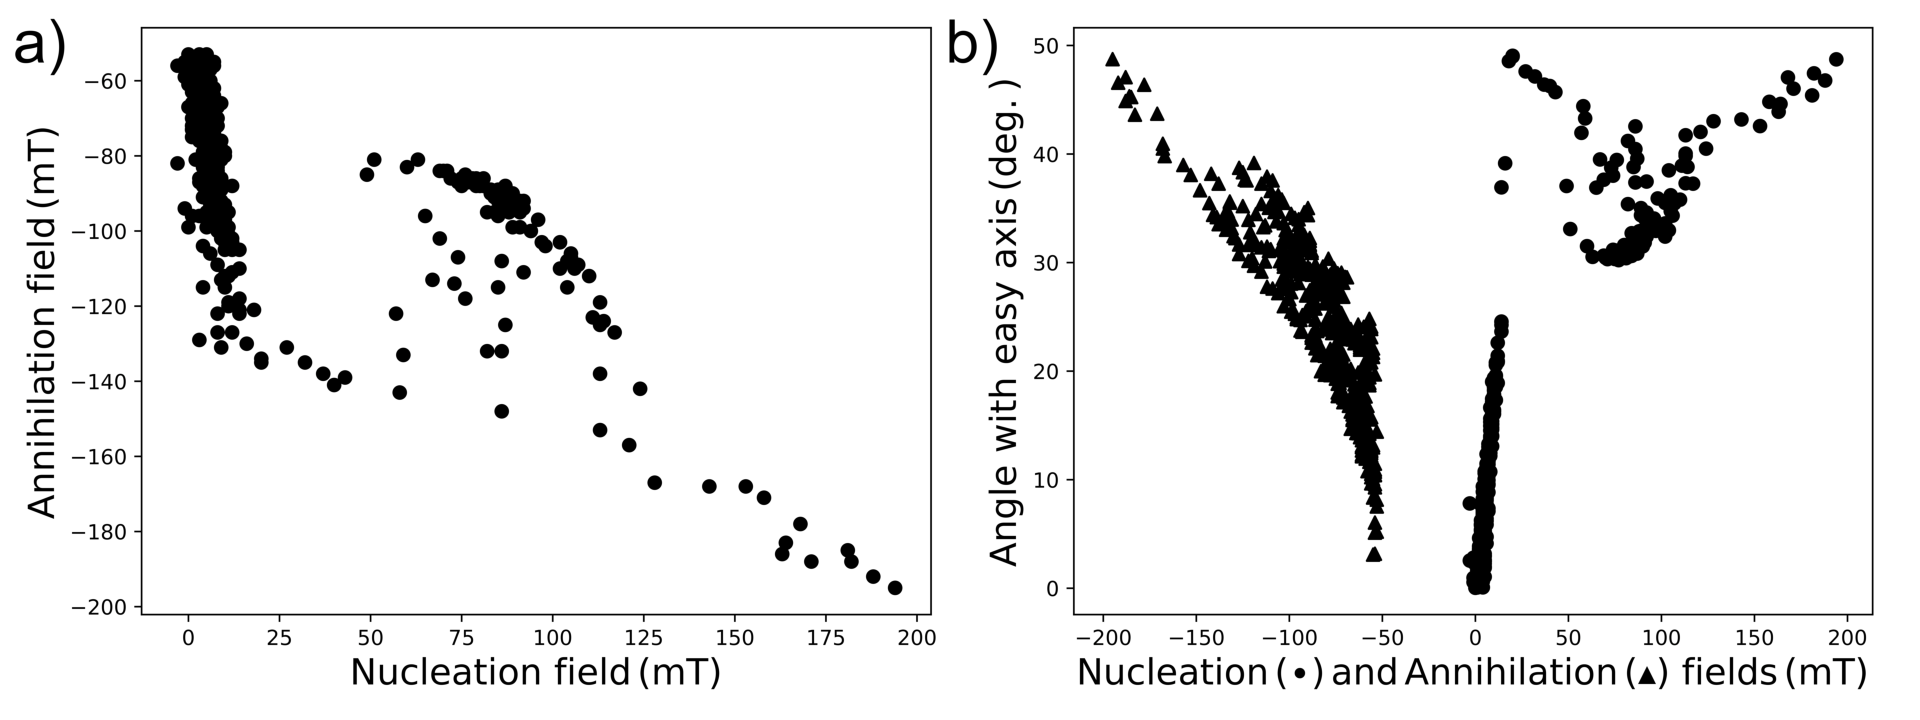
\includegraphics[width=\textwidth]{research-3/figs/FIG_08.pdf}
\caption[Vortex nucleation/annihilation fields]{Vortex nucleation/annihilation fields. a) Scatter plot of annihilation field against nucleation field. Three trends are observed depending on whether the nucleated/annihilated vortex has an easy, hard or other alignment. b) Vortex core angle with an easy direction against the nucleation/annihilation fields (circles, triangles respectively).}
\label{FIG_08}
\end{figure}
There is a large spread in the vortex nucleation and annihilation fields on the hysteresis curve (Fig. \ref{FIG_08}). Particles with hard axes alignment close to the applied field nucleate hard-aligned vortices for fields as high as $\roughly 200 \mT$ and annihilate on the opposite side of the particle for equally high (absolute) values. However, these nucleation and annihilation events have a negligible contribution to the FORC diagram as the change in magnetisation of a particle nucleating/annihilating a hard-aligned vortex from/to a SD state can be as low as $1 \%$.\par

%-----------------------------------------------------
\section{Discussion}
Comparison with the coherent-rotating dipole model of \citet{ValdezGrijalva2017} shows excellent agreement (Fig. \ref{FIG_02}). This confirms the accuracy of our model using only 500 random field orientations instead of field orientations on a regular grid, which requires a very high density of field orientationes near the sphere poles.\par

The FORC diagram of the SD coherent-rotating particles shows the same general features as those obtained for weakly interacting SD particles with cubic MCA by \citet{Harrison2014}, i.e., a positive-valued ridge along the $B_c$ axis, slightly offset towards $B_u<0$ values and a tilted, negative-valued ridge on the lower half of the FORC diagram space. For these ensembles the horizontal spread along the $B_c$ axis corresponds to the density of switching fields of the differently oriented particles and the FORC distribution peak position corresponds directly to the ensemble coercivity. The negative ridge is indicative of intermediate states along the hysteresis curve and therefore, of cubic anisotropy SD particles \citep{ValdezGrijalva2017}; this contribution is potentially unique to non-interacting to weakly interacting SD particles with cubic MCA.\par

Whereas the pure SD signal produces a tight, boomerang-shaped pattern, increasing size introduces SV structures which fragment this pattern. The FORC distribution peak is moved towards higher $B_c$ values along the $B_u=0$ axis. Paradoxically, as this occurs, the bulk coercivity of the ensembles decrease (Fig. \ref{FIG_05}). This paradox has been previously observed in synthetic size-controlled samples of sub-100$\nm$ Fe dots \citep{Dumas2007}.\par

Fragmentation of the FORC diagram for non-uniformly magnetised particles was previously observed in experimental studies by \citep{Pike1999B,Dumas2007} and in numerical models by \citet{Carvallo2003}; however, these studies did not include random field orientation distributions. The trend is nevertheless clear and is representative of the complex self-interactions brought about by the nonuniform structures and the multiple vortex nucleation/annihilation fields \citep{Pike1999B}. It is difficult to compare our results to the FORC signals measured by \citet{Muxworthy2006B} and \citet{Krasa2011} for synthetic patterned magnetite as many of their FORC diagrams appear to have ``smoothed out'' the subtle features we observe, questioning the integrity of these samples.\par

\citet{Pike1999B} obtained assymetric nucleation and annihilation fields of magnetic vortices in nano-patterned Co dots; our models agree with this finding (Fig. \ref{FIG_08}). However, \citet{Pike1999B} studied elongated disc-like particles where the vortex cores were always perpendicular to the particle plane and mostly performed reversible motion from nucleation to annihilation as they traversed the particle. In this study we have demonstrated that the different features on SV FORC diagrams, are due to a variety of vortex nucleation and annihilation events, which depend on particle alignment and the presence of distinctly different vortex states.\par

Averaged-over-size FORC diagrams were obtained for flat particle size distributions between 30$\nm$ and 80$\nm$ (Fig. \ref{FIG_09}a) and between 60$\nm$ and 80$\nm$ (Fig. \ref{FIG_09}b). The diagram in Fig. \ref{FIG_09}a shows the boomerang-shaped pattern surrounded by a variety of more complex sources. This pattern is strikingly similar to the butterfly-shaped patterns observed by \citet{Dumas2007} for their samples including both SD and SV particles. The FORC distribution peak position coincides with the ensemble coercivity while still showing a somewhat strong source corresponding to the annihilation field of easy aligned vortices.\par
\begin{figure}
\centering
\includegraphics[width=\textwidth]{research-3/figs/FIG_09.pdf}
\caption[Averaged-over-size FORC diagrams and raw hysteresis curves]{Averaged-over-size FORC diagrams (SF=4) and raw hysteresis curves. Flat size distributions used for particles $30\nm \leq d \leq 80\nm$ (a, c) and particles $60\nm \leq d \leq 80\nm$ (b, d).}
\label{FIG_09}
\end{figure}
Both diagrams in Fig. \ref{FIG_09} have a significative spread in the positive $B_u$ region. This effect is purely due to domain state, not magnetostatic interactions. The peak for the SV-dominant diagram (Fig. \ref{FIG_09}b) occurs along the $B_u=0$ axis at $B_c\approx 52\mT$ showing a disconnect with the bulk coercivity of the ensemble ($B_\text{C}\approx 16\mT$). This is a departure from the usual interpretation of FORC diagram, i.e., that the FORC diagram maps the coercivity distribution. This interpretation holds for the SD coherent-rotating grains, as the peak source coincides with the value of the ensemble coercivity. It does not hold, however, for the SV grains as their coercivity decreases with size while the position of the maximum moves towards higher values of $B_c$. Instead, for SV grains the FORC distribution peak, and indeed most of the FORC diagram features, should be interpreted as vortex nucleation/annihilation fields and their irreversible motions.\par
%-----------------------------------------------------

\section{Conclusion}
A micromagnetic FEM was employed for the calculation of the FORC diagrams of non-interacting ensembles of greigite across a size range that spans the SD to SV threshold. 500 random orientations from a distribution uniform over a sector of the sphere were used for each size. This choice was found to be in excellent agreement with previous calculations for SD greigite \citep{ValdezGrijalva2017}.\par

The FORC diagrams were found to be extremely sensitive to the domain state of the particles. When even a small fraction of particles starts to nucleate vortices, e.g., $d\approx$50$\nm$, this is reflected in the FORC diagram (Fig. \ref{FIG_03}a). The same cannot be said of the Day plot which `treats' the particles up to 60$\nm$ as strictly SD (Fig. \ref{FIG_05}a). Anomalous behaviour for particles sized 62$\nm$ to 72$\nm$ consisting in an increase of the coercivity with size was found; these particles plot in an unexpected region of the Day plot. The anomaly disappears for particles $>72\nm$, and when $d \geq 76\nm$ they appear in the region usually attributed to PSD grains.\par

Detailed analysis of the FORC diagram and micromagnetic solutions of $d=80\nm$ particles reveals the meaning of the FORC diagram for SV ensembles as a map of vortex nucleation/annihilation fields. Previous notions on how the FORC diagrams should be interpreted as a coercivity distribution need to be updated. For SD particles, the typical interpretation of the peak position coinciding with the coercivity of the sample holds; however, for SV-dominated samples, the position of the peak occurs at a value much higher than the bulk coercivity of the sample.\par
%-----------------------------------------------------

\renewcommand\bibname{{References}}
\bibliographystyle{elsarticle-harv}
\bibliography{references}

